\documentclass[tikz,margin=10pt]{standalone}
\usetikzlibrary{positioning}

\tikzset{pics/gear/.style n args={3}{
code={
    \def\modu{#1}
    \def\Zb{#2}
    \def\AngleA{#3}

    \pgfmathsetmacro{\Rpr}{\Zb*\modu/1.2}
    \pgfmathsetmacro{\Rb}{\Rpr*cos(\AngleA)}
    \pgfmathsetmacro{\Rt}{\Rpr+\modu}
    \pgfmathsetmacro{\Rp}{\Rpr-0.6*\modu}
    \pgfmathsetmacro{\AngleT}{pi/180*acos(\Rb/\Rt)}
    \pgfmathsetmacro{\AnglePr}{pi/180*acos(\Rb/\Rpr)}
    \pgfmathsetmacro{\demiAngle}{180/\Zb}
    \pgfmathsetmacro{\Angledecal}{(\demiAngle-2*\AnglePr)/2}

    \path[pic actions] foreach \zz in{1,...,\Zb}{
        \ifnum\zz=1
            % don't use a lineto in the first iteration
            (\zz/\Zb*360-\Angledecal:\Rp)
        \else
            -- (\zz/\Zb*360-\Angledecal:\Rp)
        \fi
        to[bend right=\demiAngle]
        (\zz/\Zb*360+\Angledecal:\Rp)
        --
        plot[domain=-0:\AngleT,smooth,variable=\t]
            ({{180/pi*(-\t+tan(180/pi*\t)) +\zz/\Zb*360+\Angledecal}:\Rb/cos(180/pi*\t)})
        %
        to[bend right=\demiAngle]
            ({{180/pi*(\AngleT+tan(180/pi*-\AngleT)) +(\zz+1)/\Zb*360-\Angledecal}:
            \Rb/cos(180/pi*-\AngleT)})
        --
        plot[domain=-\AngleT:-0,smooth,variable=\t]
        ({{180/pi*(-\t+tan(180/pi*\t)) +(\zz+1)/\Zb*360-\Angledecal}:\Rb/cos(180/pi*\t)})
    } -- cycle;
}
}}

\begin{document}
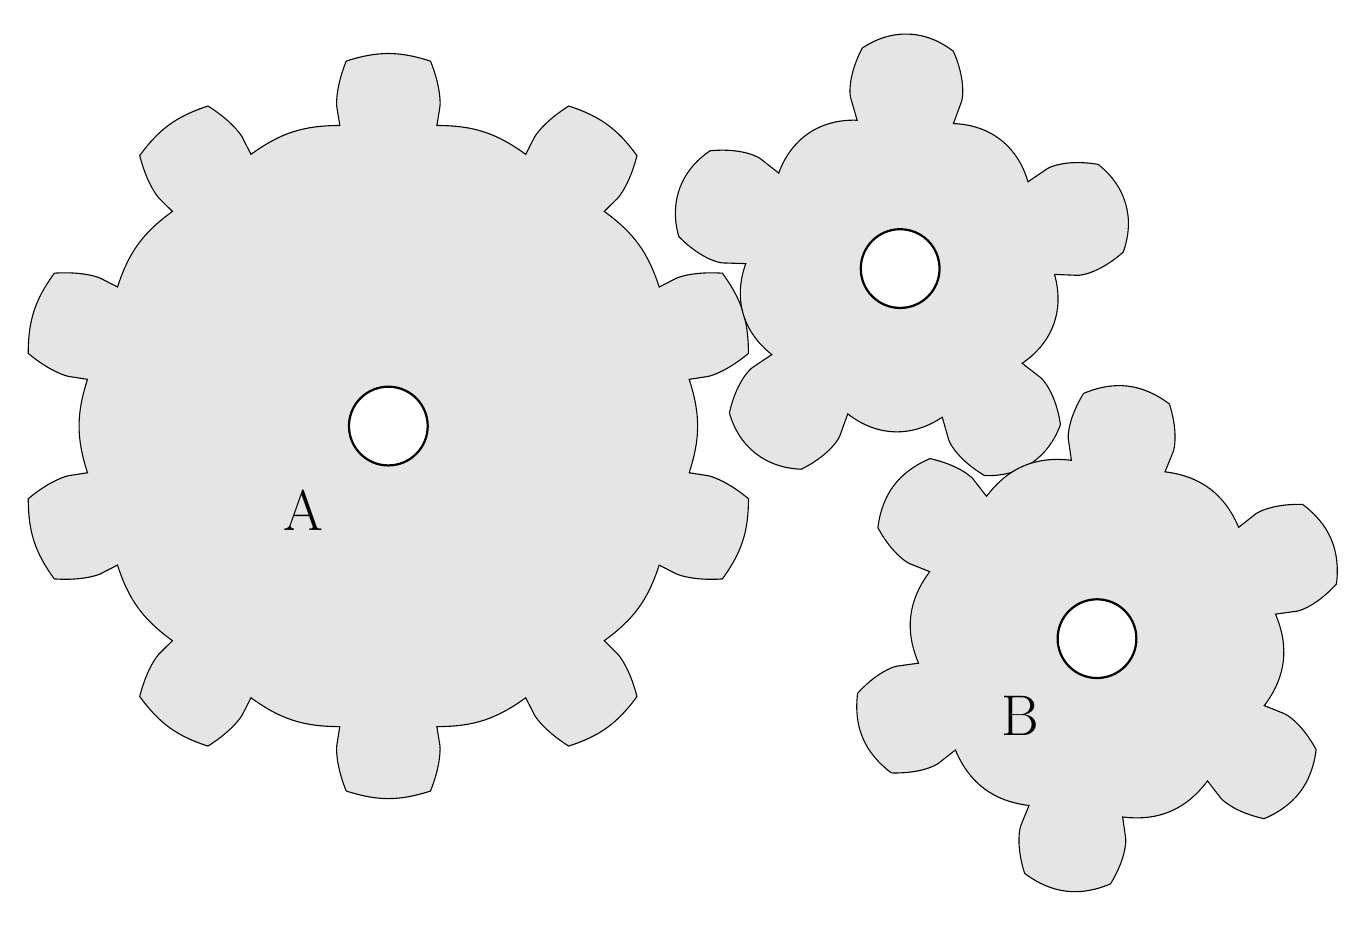
\begin{tikzpicture}[scale=1]
    % - param #1: modulus of wheel
    % - param #2: number of teeth
    % - param #3: angle
    % - param #1 and #3 must be equal for gears to mesh
    % draw the cogwheels
    \coordinate (A) at (0,0);
    \coordinate (B) at (9,-2.7);
    \coordinate (C) at (6.5,2);
    \pic[draw,fill=gray!20,rotate=0] at (A) {gear={0.5}{10}{10}};
    \pic[draw,fill=gray!20,rotate=-20] at (C) {gear={0.55}{5}{10}};
    \pic[draw,fill=gray!20,rotate=-7] at (B) {gear={0.52}{6}{10}};
    % draw the center of the cogwheel
    \foreach \p in {(A),(B),(C)} \fill [thick,draw=black,fill=white] \p circle(0.5cm); 
    % add labels
    \node[thick,below left= 0.7cm and 0.7cm of A]{\huge A};
    \node[thick,below left= 0.6cm and 0.6cm of B]{\huge B};
\end{tikzpicture}

\end{document}